%\{ {\it  sp1d\_ch3\_1.tex} \}

Consider the problem (\ref{poisson1}) in the viewpoint of convergence having solution $u \in H^k(\Omega)= \{u|\sum_{|j|\le k }\frac{d^j}{dx^j} \in L^2(\Omega) \}$.

Assuming a discretisation on a uniform domain of equi-spaced subinterval of size $h$, the general error estimate in the norm $||\cdot||_{H^k(\Omega)}$ for the h-and p-type extension process can be written as \cite{Karniadarkis}

\begin{equation}
\label{hprelation}
||\epsilon||_{H^k(\Omega)} \le CH^{\mu-1}P^{-(k-1)}||u||_{H^k(\Omega)},
\end{equation}
where $\epsilon = u - u^{\delta}, \mu = \mbox{min}(k, P+1)$, and $C$ is independent of $h$, $P$ and $u$, but depends on $k$.

This means if a solution $u$ lies in  $H^k(\Omega)$ for sufficiently large $k > P+1$, then this error estimate shows that we can achieve exponential convergence as we increase the polynomial order P. Also in particular to h-extension process, the error respect to norm $||\cdot||_{H^1(\Omega)}$ satisfies:
\begin{equation}
\label{hrelation} ||\epsilon||_{H^1(\Omega)} \le K_1Ch.
\end{equation}
From \cite{Karniadarkis}, we see that the slope of the h-type extension process is related to the minimum of $P+1$ and the smoothness $k$ of the solution. In our experiment, since we take the example having smooth solutions, we can see the slope of h-type extension graph of errors to be very close to $P+1$.

\subsection {H/P Convergence Test for One-dimensional Solution}

In this section we present the result of convergence in both $h$ refinement and $p$ refinement with the following steady-state Poisson differential equation:
\begin{equation}
\label{pois_sin}
\frac{d^2}{dx^2} u(x) = \sin(\pi x),
\end{equation}
for all x in $[0, 1]$ with zero Dirichlet and Neumann boundary conditions.

The numerical and exact solutions by the solver we developed is shown in figure (\ref{sinsol}).

\begin{figure}[h]
    \begin{center}
    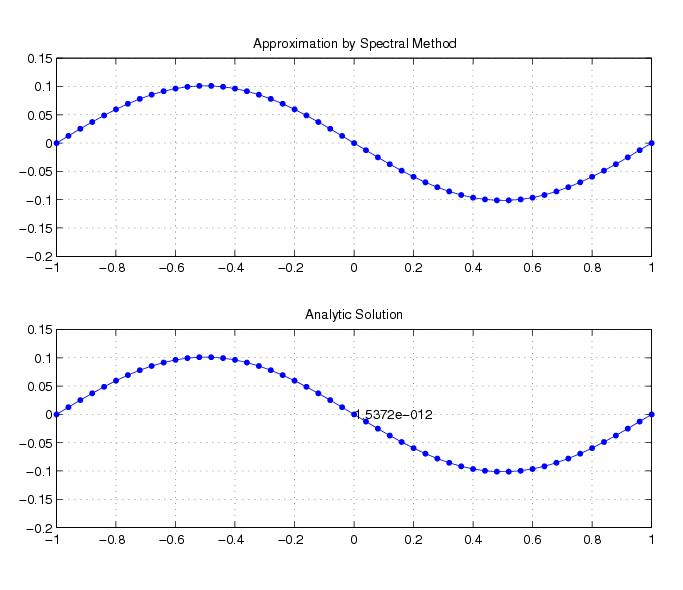
\epsfig{file = figs_dn/sinDN_O15.eps, width = 5cm}
    \caption{\label{sinsol}Numerical and exact solution of equation (\ref{pois_sin}) with polynomial order $P=15$}
    \end{center}
\end{figure}

\begin{itemize}

\item {Convergence of h-type extension for equation (\ref{pois_sin})}

This test is to validate the relation between size of element and the accuracy of approximation. We apply equi-distance elements and investigate the movement of error scale. As shown in Figure (\ref{sinDNconv}), the smaller are the elements, the more exact is the solution.

As we see the relationship (\ref{hrelation}) in the theory, the slope of convergence graph shows slope 4, 5, and 6 for the polynomial order 3, 4, and 5 respectively. the exact outcome is shown in left table of Table (\ref{hconv2t}).

\item {Convergence of p-type extension for equation (\ref{pois_sin})}

Since the exact solution is infinite sum of polynomial function, with finite order of interpolating trial functions cannot reach the ideal convergence. But conversely, this also shows the fact that the convergence stay in steady state before the error reached the machine precision range. As shown in right figure of Figure (\ref{sinDNconv}), it proves the fact that is explained in equation (\ref{hprelation}).

\end{itemize}

\begin{figure}[h]
\begin{center}
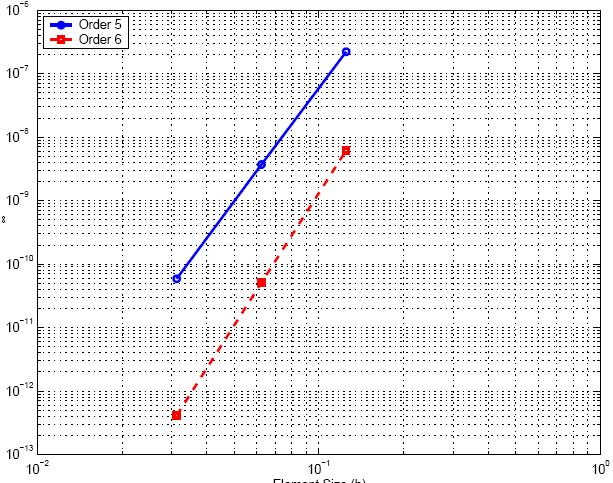
\epsfig{file = figs_dn/sinDNhconv.eps, width = 8.3cm}
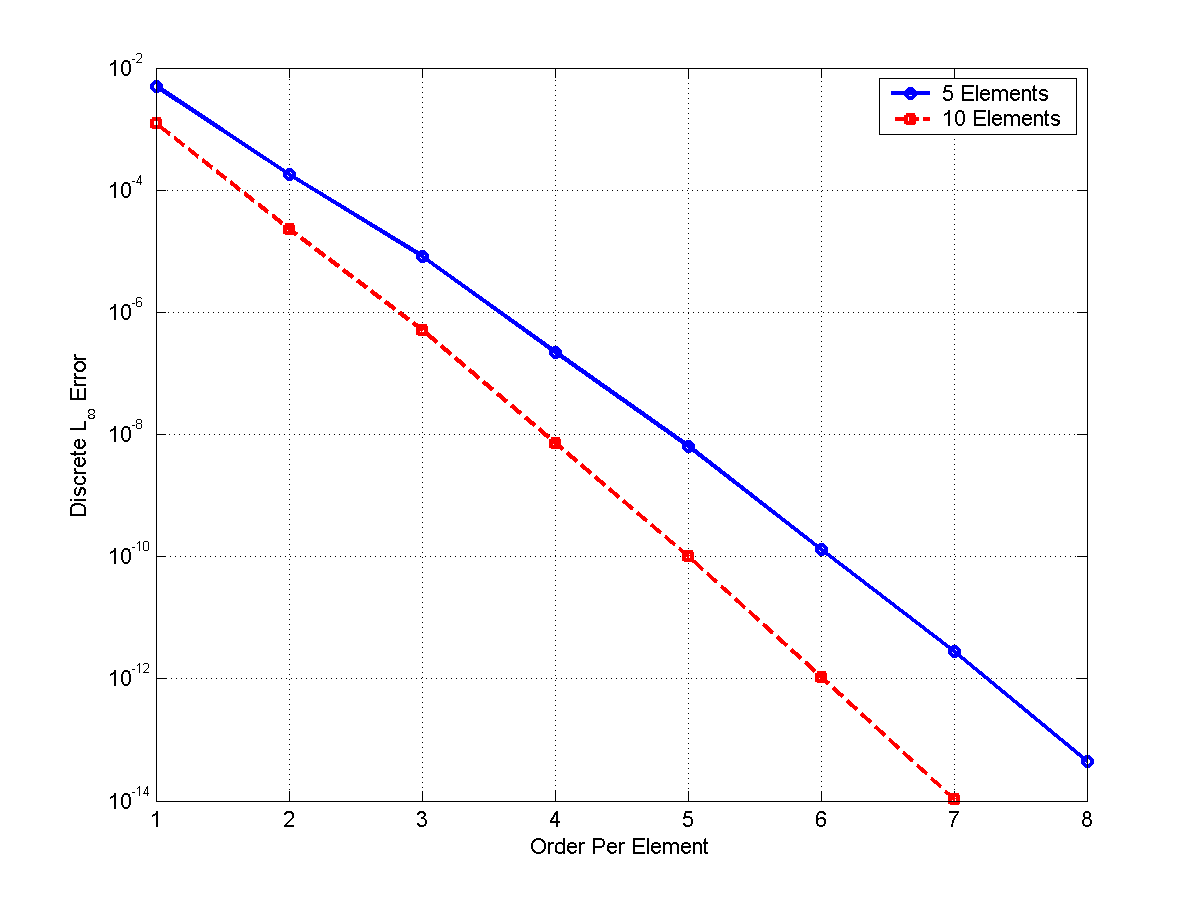
\epsfig{file = figs_dn/sinDNpconv.eps, width = 8.3cm}
\caption{\label{sinDNconv}
(Left)Convergence with respect to discrete $L^{\infty}$ norm as a function of size of elements. This test is performed using the h-type extension with fixed polynomial order 3, 4, and 5 respectively. Error on the Log-Log axis is demonstrating the algebraic convergence of the h-type extension.
(Right)Convergence w.r.t. $L^{\infty}$ norm as a function of size of polynomial order in semi-Log plot. It shows the exponential convergence of p-type extension for smooth solution. Two tests are performed for p-type extension with element length $0.2$ and $0.1$.
}
\end{center}
\end{figure}

\begin{table}[h]
\centering \caption{\label{hconv2t} This table shows the convergence of h-type (left) and p-type (right) resolution control done above Figure (\ref{sinDNconv}). We can see the slopes of each order $P$ is $P+1$ }
\begin{tabular}{|c|c|c|} \hline
    Polynomial order&Error($L^{\infty}$)&Slope   \\ \hline \hline
    3&$1.1620e-012$ &$4.0024$ \\ \hline
    4&$4.6629e-014$ &$4.9877$ \\ \hline
    5&$9.7367e-014$ &$5.9775$ \\ \hline
\end{tabular}
\hspace{.5in}
\begin{tabular}{|c|c|} \hline
    &\multicolumn{1}{|c|}{Error}\\
    \raisebox{0.5\baselineskip}%
    {Element Size}&($L^{\infty}$) \\ \hline \hline
    0.2&$8.3267e-016$  \\ \hline
    0.1&$6.6613e-016$  \\ \hline
\end{tabular}

\end{table}
